%%%%%%%%%%%%%%%%%%%%%%%%%%%%%%%%%%%%%%%%%
% Beamer Presentation
% LaTeX Template
% Version 1.0 (10/11/12)
%
% This template has been downloaded from:
% http://www.LaTeXTemplates.com
%
% License:
% CC BY-NC-SA 3.0 (http://creativecommons.org/licenses/by-nc-sa/3.0/)
%
%%%%%%%%%%%%%%%%%%%%%%%%%%%%%%%%%%%%%%%%%

%----------------------------------------------------------------------------------------
%	PACKAGES AND THEMES
%----------------------------------------------------------------------------------------

\documentclass{beamer}

\mode<presentation> {

% The Beamer class comes with a number of default slide themes
% which change the colors and layouts of slides. Below this is a list
% of all the themes, uncomment each in turn to see what they look like.

\usetheme{Boadilla}
\usetheme[numbering=fraction,progressbar=foot]{metropolis}
% Install metropolis from here: https://github.com/matze/mtheme
}

\usepackage[utf8]{inputenc}
\usepackage{graphicx} 
\usepackage{booktabs} 
\usepackage{hyperref}
\usepackage{listings}
\usepackage{color}
\usepackage[font=small,labelfont=bf]{caption}
\usepackage{subfig}
\usepackage{appendixnumberbeamer}

\definecolor{dkgreen}{rgb}{0,0.6,0}
\definecolor{gray}{rgb}{0.5,0.5,0.5}
\definecolor{mauve}{rgb}{0.58,0,0.82}

\lstset{
  language=Java,
  showstringspaces=false,
  columns=flexible,
  basicstyle={\small\ttfamily},
  numbers=none,
  numberstyle=\tiny\color{gray},
  keywordstyle=\color{blue},
  commentstyle=\color{dkgreen},
  stringstyle=\color{mauve},
  breaklines=true,
  breakatwhitespace=true,
  tabsize=3
}

%----------------------------------------------------------------------------------------
%	TITLE PAGE
%----------------------------------------------------------------------------------------

\title[]{Introduction to Robotics} 

\author[Santosh Thoduka]{Santosh Thoduka}
\institute[HBRS]{Hochschule Bonn Rhein Sieg}

\date{September 10, 2019}

\begin{document}
\setbeamertemplate{frametitle}[default][center]
\setbeamertemplate{caption}[numbered]
\setbeamertemplate{bibliography item}{\insertbiblabel}
\captionsetup[subfigure]{labelformat=empty}
\setbeamerfont{footnote}{size=\tiny}

\begin{frame}[plain]
\addtocounter{framenumber}{-1}
\maketitle
\end{frame}

%%%%%%%%%%%%%%%%%%%%%%%%%%%%%%%%%%%%%%%%%%%%%%%%%%%%
\begin{frame}
\frametitle{Introduction}
\begin{itemize}
    \item Motivation: to introduce you to high-level keywords and concepts in robotics
    \item Outline: watch videos and create a mindmap on the board
    \item This is \emph{not} a lecture; it is a discussion
    \item Further reading: Springer Handbook of Robotics (https://www.springer.com/de/book/9783540303015)
\end{itemize}

\end{frame}

%%%%%%%%%%%%%%%%%%%%%%%%%%%%%%%%%%%%%%%%%%%%%%%%%%%%
\begin{frame}
\frametitle{Videos!}
\begin{itemize}
\item <1-> b-it-bots@Work Basic Transportation Test
\item <2-> Tech United Mid-sized League soccer
\item <3-> b-it-bots@Home Storing Groceries
\item <4-> Australian Centre for Robotic Vision Amazon Picking Challenge
\item <5-> Nimbro at MBZIRC 2017
\end{itemize}

\end{frame}

%%%%%%%%%%%%%%%%%%%%%%%%%%%%%%%%%%%%%%%%%%%%%%%%%%%%
\begin{frame}[standout]
     Domains
\end{frame}

%%%%%%%%%%%%%%%%%%%%%%%%%%%%%%%%%%%%%%%%%%%%%%%%%%%%
\begin{frame}
\frametitle{Domains}
\begin{itemize}
    \item Navigation
    \item Sensing
    \item Manipulation
    \item Task Planning
\end{itemize}
\end{frame}

%%%%%%%%%%%%%%%%%%%%%%%%%%%%%%%%%%%%%%%%%%%%%%%%%%%%
\begin{frame}[standout]
     Navigation
\end{frame}


%%%%%%%%%%%%%%%%%%%%%%%%%%%%%%%%%%%%%%%%%%%%%%%%%%%%
\begin{frame}
\frametitle{Navigation}
\begin{itemize}
    \item <1->World model
    \item <2->SLAM
    \item <3->Path planning
    \item <4->Motion planning - how do robots move?
    \item <5->Obstacle avoidance
    \item <6->What about aerial, underwater and legged robots?
\end{itemize}

\onslide<2->
{\footnotesize
Videos:
\begin{itemize}
\item <2->{[06-Mapping]}
\end{itemize}}
\end{frame}

\begin{frame}
\frametitle{OpenStreetMap}
\begin{figure}[H]
     \centering
     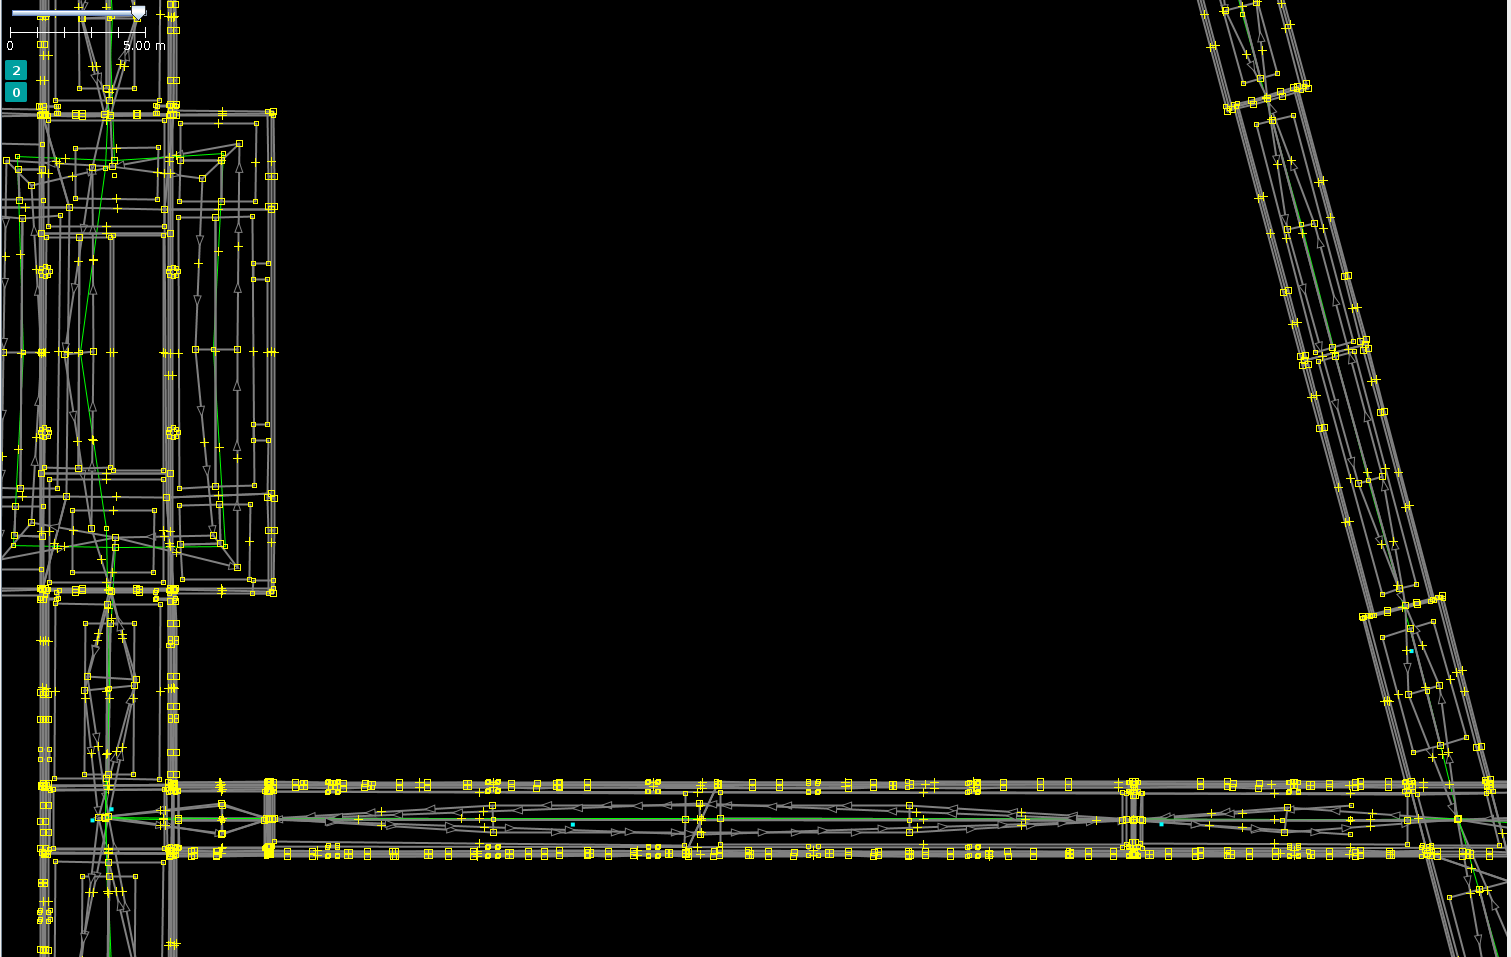
\includegraphics[width=0.95\textwidth]{images/OSM.png}
     \caption{Indoor OpenStreetMap of university~\cite{Naik2019}}
     \label{fig:pick}
\end{figure}
\end{frame}

%%%%%%%%%%%%%%%%%%%%%%%%%%%%%%%%%%%%%%%%%%%%%%%%%%%%
\begin{frame}[standout]
     Sensing
\end{frame}

%%%%%%%%%%%%%%%%%%%%%%%%%%%%%%%%%%%%%%%%%%%%%%%%%%%%
\begin{frame}
\frametitle{Sensors}
\begin{itemize}
    \item Laser scanner
    \item 2D camera
    \item 3D camera
    \item Sonar
    \item IMU
    \item Microphone
    \item Tactile
    \item Force and torque
\end{itemize}
\end{frame}

%%%%%%%%%%%%%%%%%%%%%%%%%%%%%%%%%%%%%%%%%%%%%%%%%%%%
\begin{frame}[standout]
     Vision
\end{frame}
%%%%%%%%%%%%%%%%%%%%%%%%%%%%%%%%%%%%%%%%%%%%%%%%%%%%
\begin{frame}
\frametitle{Sensing}
\framesubtitle{Vision}
\begin{itemize}
    \item <1->Object detection and recognition
    \item <2->Person / face detection and recognition
    \item <3->Visual servoing
    \item <4->Motion detection
    \item <5->Tracking
    \item <6->Action recognition
\end{itemize}

\onslide<1->
{\footnotesize
Videos:
\begin{itemize}
\item <1->{[07-3D-Detection]}
\item <1->{[08-2D-Segmentation]}
\item <1->{[09-2D-Detection]}
\item <3->{[10-Visual-Servoing]}
\item <6->{[11-Action-Recognition]}
\end{itemize}}
\end{frame}

%%%%%%%%%%%%%%%%%%%%%%%%%%%%%%%%%%%%%%%%%%%%%%%%%%%%
\begin{frame}[standout]
     Sound
\end{frame}
%%%%%%%%%%%%%%%%%%%%%%%%%%%%%%%%%%%%%%%%%%%%%%%%%%%%
\begin{frame}
\frametitle{Sensing}
\framesubtitle{Sound}
\begin{itemize}
    \item <1->Speech recognition
    \item <2->Speaker identification
    \item <3->Sound localization
    \item <4->Anomalous sound classification
\end{itemize}
\end{frame}

%%%%%%%%%%%%%%%%%%%%%%%%%%%%%%%%%%%%%%%%%%%%%%%%%%%%
\begin{frame}
\frametitle{Sensing}
\begin{itemize}
    \item <1->Force / load sensing
    \item <2->Tactile
        \begin{itemize}
            \item Compliant motion
            \item Grasp verification
        \end{itemize}
    \item <3->Inertial
    \item <4->Range
\end{itemize}
\end{frame}

%%%%%%%%%%%%%%%%%%%%%%%%%%%%%%%%%%%%%%%%%%%%%%%%%%%%
\begin{frame}[standout]
     Manipulation
\end{frame}


%%%%%%%%%%%%%%%%%%%%%%%%%%%%%%%%%%%%%%%%%%%%%%%%%%%%
\begin{frame}
\frametitle{Manipulation}
\begin{itemize}
    \item <1->Model identification
    \item <2->Motion planning
    \item <3->Motion control
    \item <4->Force control
    \item <5->Grasping
    \item <6->Insertion
\end{itemize}

\onslide<2->
{\footnotesize
Videos:
\begin{itemize}
\item <2->{[12-Motion-Planning]}
\item <4->{[13-Force-Control]}
\item <6->{[14-Peg-in-Hole-Task]}
\end{itemize}}
\end{frame}

%%%%%%%%%%%%%%%%%%%%%%%%%%%%%%%%%%%%%%%%%%%%%%%%%%%%
\begin{frame}[standout]
     Planning
\end{frame}

%%%%%%%%%%%%%%%%%%%%%%%%%%%%%%%%%%%%%%%%%%%%%%%%%%%%
\begin{frame}
\frametitle{Task Planning}
\framesubtitle{Hardcoded state machine for Basic Transportation Task}
\begin{figure}[H]
     \centering
     \includegraphics[width=0.5\textwidth]{images/BTT.png}
     \caption{Basic Transportation Task~\cite{Lima}}
     \label{fig:btt}
\end{figure}
\end{frame}

%%%%%%%%%%%%%%%%%%%%%%%%%%%%%%%%%%%%%%%%%%%%%%%%%%%%
\begin{frame}
\frametitle{Task Planning}
\framesubtitle{Hardcoded state machine for \texttt{pick object}}
\begin{figure}[H]
     \centering
     \includegraphics[width=0.35\textwidth]{images/Pick.png}
     \caption{Pick object~\cite{Lima}}
     \label{fig:pick}
\end{figure}
\end{frame}

%%%%%%%%%%%%%%%%%%%%%%%%%%%%%%%%%%%%%%%%%%%%%%%%%%%%
\begin{frame}[fragile]
\frametitle{Task Planning}
\framesubtitle{Sample plan for Basic Transportation Task}
    \begin{verbatim}
        (move_base youbot-brsu start ws02)
        (perceive youbot-brsu ws02)
        (pick youbot-brsu ws02 bearing-00)
        (stage youbot-brsu platform_left bearing-00)
        (move_base youbot-brsu ws02 ws04)
        (unstage youbot-brsu platform_left bearing-00)
        (place youbot-brsu ws04 bearing-00)
    \end{verbatim}
\end{frame}

%%%%%%%%%%%%%%%%%%%%%%%%%%%%%%%%%%%%%%%%%%%%%%%%%%%%
\begin{frame}
\frametitle{Task Planning}
\framesubtitle{Sample plan for making peppermint tea}
\begin{figure}[H]
     \centering
     \includegraphics[width=0.4\textwidth]{images/bring_me_tea.png}
     \caption{Plan for making peppermint tea~\cite{Awaad}}
     \label{fig:tea}
\end{figure}
\end{frame}

%%%%%%%%%%%%%%%%%%%%%%%%%%%%%%%%%%%%%%%%%%%%%%%%%%%%
\begin{frame}
\frametitle{Software}
\begin{itemize}
    \item <1->Languages: C++, Python, Java
    \item <2->Frameworks: ROS, Orocos, Fawkes
    \item <3->Simulators: Gazebo, Stage, V-Rep, OpenRAVE
    \item <4->Useful libraries: KDL\footnote{https://wiki.ros.org/kdl}, OpenCV, PCL, ZeroMQ, etc.
\end{itemize}
\end{frame}


%%%%%%%%%%%%%%%%%%%%%%%%%%%%%%%%%%%%%%%%%%%%%%%%%%%%
\begin{frame}
\frametitle{Some other topics}
\begin{itemize}
    \item <1->Natural language processing
    \item <2->Fault detection and error recovery
    \item <3->Learning
    \item <4->Sensor fusion
    \item <5->Probabilistic reasoning
    \item <6->Active perception
    \item <7->Multi-robot systems
    \item <8->Logging and databases
    \item <9->Communication
    \item <10->Human-robot interaction
    \item <11->User interfaces
    \item <12->Learning by demonstration
\end{itemize}
\end{frame}

%%%%%%%%%%%%%%%%%%%%%%%%%%%%%%%%%%%%%%%%%%%%%%%%%%%%
\appendix
\begin{frame}[allowframebreaks]
        \frametitle{References}
        \bibliographystyle{ieeetr}
        \bibliography{BibTex.bib}
\end{frame}

%%%%%%%%%%%%%%%%%%%%%%%%%%%%%%%%%%%%%%%%%%%%%%%%%%%%
\begin{frame}[standout]
     The End!
\end{frame}



%%%%%%%%%%%%%%%%%%%%%%%%%%%%%%%%%%%%%%%%%%%%%%%%%%%%
\end{document} 
